% Options for packages loaded elsewhere
\PassOptionsToPackage{unicode}{hyperref}
\PassOptionsToPackage{hyphens}{url}
%
\documentclass[
]{article}
\usepackage{amsmath,amssymb}
\usepackage{lmodern}
\usepackage{ifxetex,ifluatex}
\ifnum 0\ifxetex 1\fi\ifluatex 1\fi=0 % if pdftex
  \usepackage[T1]{fontenc}
  \usepackage[utf8]{inputenc}
  \usepackage{textcomp} % provide euro and other symbols
\else % if luatex or xetex
  \usepackage{unicode-math}
  \defaultfontfeatures{Scale=MatchLowercase}
  \defaultfontfeatures[\rmfamily]{Ligatures=TeX,Scale=1}
\fi
% Use upquote if available, for straight quotes in verbatim environments
\IfFileExists{upquote.sty}{\usepackage{upquote}}{}
\IfFileExists{microtype.sty}{% use microtype if available
  \usepackage[]{microtype}
  \UseMicrotypeSet[protrusion]{basicmath} % disable protrusion for tt fonts
}{}
\makeatletter
\@ifundefined{KOMAClassName}{% if non-KOMA class
  \IfFileExists{parskip.sty}{%
    \usepackage{parskip}
  }{% else
    \setlength{\parindent}{0pt}
    \setlength{\parskip}{6pt plus 2pt minus 1pt}}
}{% if KOMA class
  \KOMAoptions{parskip=half}}
\makeatother
\usepackage{xcolor}
\IfFileExists{xurl.sty}{\usepackage{xurl}}{} % add URL line breaks if available
\IfFileExists{bookmark.sty}{\usepackage{bookmark}}{\usepackage{hyperref}}
\hypersetup{
  pdftitle={SVD image compression},
  pdfauthor={Andrés Mejía Rodríguez},
  hidelinks,
  pdfcreator={LaTeX via pandoc}}
\urlstyle{same} % disable monospaced font for URLs
\usepackage[margin=1in]{geometry}
\usepackage{color}
\usepackage{fancyvrb}
\newcommand{\VerbBar}{|}
\newcommand{\VERB}{\Verb[commandchars=\\\{\}]}
\DefineVerbatimEnvironment{Highlighting}{Verbatim}{commandchars=\\\{\}}
% Add ',fontsize=\small' for more characters per line
\usepackage{framed}
\definecolor{shadecolor}{RGB}{248,248,248}
\newenvironment{Shaded}{\begin{snugshade}}{\end{snugshade}}
\newcommand{\AlertTok}[1]{\textcolor[rgb]{0.94,0.16,0.16}{#1}}
\newcommand{\AnnotationTok}[1]{\textcolor[rgb]{0.56,0.35,0.01}{\textbf{\textit{#1}}}}
\newcommand{\AttributeTok}[1]{\textcolor[rgb]{0.77,0.63,0.00}{#1}}
\newcommand{\BaseNTok}[1]{\textcolor[rgb]{0.00,0.00,0.81}{#1}}
\newcommand{\BuiltInTok}[1]{#1}
\newcommand{\CharTok}[1]{\textcolor[rgb]{0.31,0.60,0.02}{#1}}
\newcommand{\CommentTok}[1]{\textcolor[rgb]{0.56,0.35,0.01}{\textit{#1}}}
\newcommand{\CommentVarTok}[1]{\textcolor[rgb]{0.56,0.35,0.01}{\textbf{\textit{#1}}}}
\newcommand{\ConstantTok}[1]{\textcolor[rgb]{0.00,0.00,0.00}{#1}}
\newcommand{\ControlFlowTok}[1]{\textcolor[rgb]{0.13,0.29,0.53}{\textbf{#1}}}
\newcommand{\DataTypeTok}[1]{\textcolor[rgb]{0.13,0.29,0.53}{#1}}
\newcommand{\DecValTok}[1]{\textcolor[rgb]{0.00,0.00,0.81}{#1}}
\newcommand{\DocumentationTok}[1]{\textcolor[rgb]{0.56,0.35,0.01}{\textbf{\textit{#1}}}}
\newcommand{\ErrorTok}[1]{\textcolor[rgb]{0.64,0.00,0.00}{\textbf{#1}}}
\newcommand{\ExtensionTok}[1]{#1}
\newcommand{\FloatTok}[1]{\textcolor[rgb]{0.00,0.00,0.81}{#1}}
\newcommand{\FunctionTok}[1]{\textcolor[rgb]{0.00,0.00,0.00}{#1}}
\newcommand{\ImportTok}[1]{#1}
\newcommand{\InformationTok}[1]{\textcolor[rgb]{0.56,0.35,0.01}{\textbf{\textit{#1}}}}
\newcommand{\KeywordTok}[1]{\textcolor[rgb]{0.13,0.29,0.53}{\textbf{#1}}}
\newcommand{\NormalTok}[1]{#1}
\newcommand{\OperatorTok}[1]{\textcolor[rgb]{0.81,0.36,0.00}{\textbf{#1}}}
\newcommand{\OtherTok}[1]{\textcolor[rgb]{0.56,0.35,0.01}{#1}}
\newcommand{\PreprocessorTok}[1]{\textcolor[rgb]{0.56,0.35,0.01}{\textit{#1}}}
\newcommand{\RegionMarkerTok}[1]{#1}
\newcommand{\SpecialCharTok}[1]{\textcolor[rgb]{0.00,0.00,0.00}{#1}}
\newcommand{\SpecialStringTok}[1]{\textcolor[rgb]{0.31,0.60,0.02}{#1}}
\newcommand{\StringTok}[1]{\textcolor[rgb]{0.31,0.60,0.02}{#1}}
\newcommand{\VariableTok}[1]{\textcolor[rgb]{0.00,0.00,0.00}{#1}}
\newcommand{\VerbatimStringTok}[1]{\textcolor[rgb]{0.31,0.60,0.02}{#1}}
\newcommand{\WarningTok}[1]{\textcolor[rgb]{0.56,0.35,0.01}{\textbf{\textit{#1}}}}
\usepackage{graphicx}
\makeatletter
\def\maxwidth{\ifdim\Gin@nat@width>\linewidth\linewidth\else\Gin@nat@width\fi}
\def\maxheight{\ifdim\Gin@nat@height>\textheight\textheight\else\Gin@nat@height\fi}
\makeatother
% Scale images if necessary, so that they will not overflow the page
% margins by default, and it is still possible to overwrite the defaults
% using explicit options in \includegraphics[width, height, ...]{}
\setkeys{Gin}{width=\maxwidth,height=\maxheight,keepaspectratio}
% Set default figure placement to htbp
\makeatletter
\def\fps@figure{htbp}
\makeatother
\setlength{\emergencystretch}{3em} % prevent overfull lines
\providecommand{\tightlist}{%
  \setlength{\itemsep}{0pt}\setlength{\parskip}{0pt}}
\setcounter{secnumdepth}{-\maxdimen} % remove section numbering
\ifluatex
  \usepackage{selnolig}  % disable illegal ligatures
\fi

\title{SVD image compression}
\author{Andrés Mejía Rodríguez}
\date{11/8/2021}

\begin{document}
\maketitle

\hypertarget{introduction}{%
\subsection{Introduction}\label{introduction}}

In the following work we will explore how does compressing an image
using SVD works. For this we will take an image and see how different
compression work and how big the compression ratios are.

\hypertarget{original-image}{%
\subsection{Original Image}\label{original-image}}

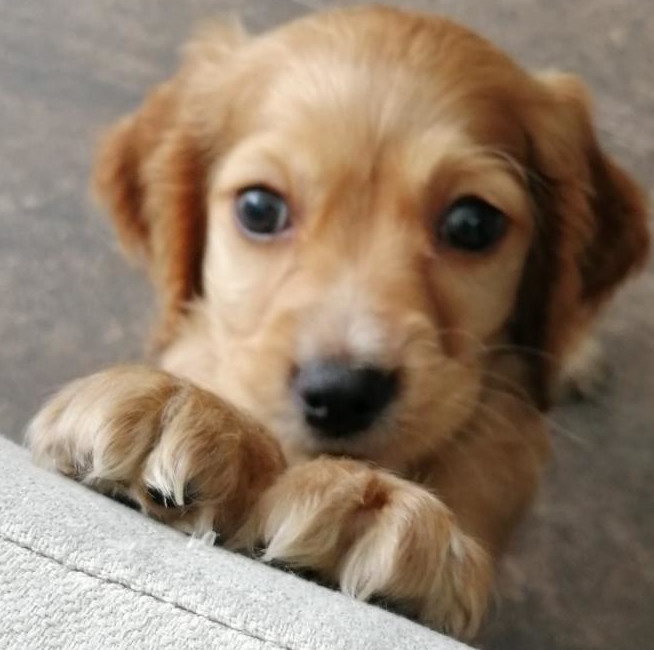
\includegraphics{blip2.jpg}

This work will be based on the above image. The picture is 654X650. We
can also check that it is a full rank matrix (650) in all 3 color spaces
using the rank command in matlab. So the original image needs

\begin{Shaded}
\begin{Highlighting}[]
\DecValTok{650}\SpecialCharTok{*}\DecValTok{654}\SpecialCharTok{*}\DecValTok{3}
\end{Highlighting}
\end{Shaded}

\begin{verbatim}
## [1] 1275300
\end{verbatim}

Different numbers for storing the whole image.

\hypertarget{compression-information}{%
\subsection{Compression Information}\label{compression-information}}

For getting the low rank compression we will use the ``compress.m'' file
modified (included in the folder) to export the image files and find the
rank of the resulting matrices.

Given that in a compressed Matrix of rank k

\[
A_k=\sum_{i=1}^k\sigma_i \vec{u_k}\vec{v_k}^t
\]

holds 1 item of information in \(\sigma_i\), items equal to the vertical
size in \(\vec{u_i}\) and items equal to the horizontal size in
\(\vec{v_i}\). Also note that this has to be done for all 3 colors so in
total we need

\[
(650+654+1)3k
\]

And we get a compression equivalent to

\[
\frac{(650+654+1)3k}{650*654*3}
\] We can see a few select values in the following table.

\begin{Shaded}
\begin{Highlighting}[]
\NormalTok{V}\OtherTok{=}\FunctionTok{data.frame}\NormalTok{(}\AttributeTok{rank=}\FunctionTok{c}\NormalTok{(}\DecValTok{1}\NormalTok{,}\DecValTok{2}\NormalTok{,}\DecValTok{10}\NormalTok{,}\DecValTok{40}\NormalTok{,}\DecValTok{100}\NormalTok{,}\DecValTok{325}\NormalTok{,}\DecValTok{650}\NormalTok{))}
\NormalTok{V }\SpecialCharTok{\%\textless{}\textgreater{}\%} \FunctionTok{mutate}\NormalTok{(}\AttributeTok{comp\_data=}\NormalTok{(}\DecValTok{650}\SpecialCharTok{+}\DecValTok{654}\SpecialCharTok{+}\DecValTok{1}\NormalTok{)}\SpecialCharTok{*}\DecValTok{3}\SpecialCharTok{*}\NormalTok{rank,}\AttributeTok{comp\_rate=}\NormalTok{comp\_data}\SpecialCharTok{/}\NormalTok{(}\DecValTok{650}\SpecialCharTok{*}\DecValTok{654}\SpecialCharTok{*}\DecValTok{3}\NormalTok{))}
\NormalTok{V}
\end{Highlighting}
\end{Shaded}

\begin{verbatim}
##   rank comp_data   comp_rate
## 1    1      3915 0.003069866
## 2    2      7830 0.006139732
## 3   10     39150 0.030698659
## 4   40    156600 0.122794637
## 5  100    391500 0.306986591
## 6  325   1272375 0.997706422
## 7  650   2544750 1.995412844
\end{verbatim}

Note that when using half the rank uses almost the same information than
the image itself and using the full rank uses almost twice as much as
the original image.

\hypertarget{image-comparision}{%
\subsection{Image comparision}\label{image-comparision}}

The following shows the results of compressing the image using the first
40 SVD

\includegraphics{ani.gif}

We can see that we mostly get a recognizable picture but lose detail for
example in the front paws.

Using 100 rank we get the following picture:

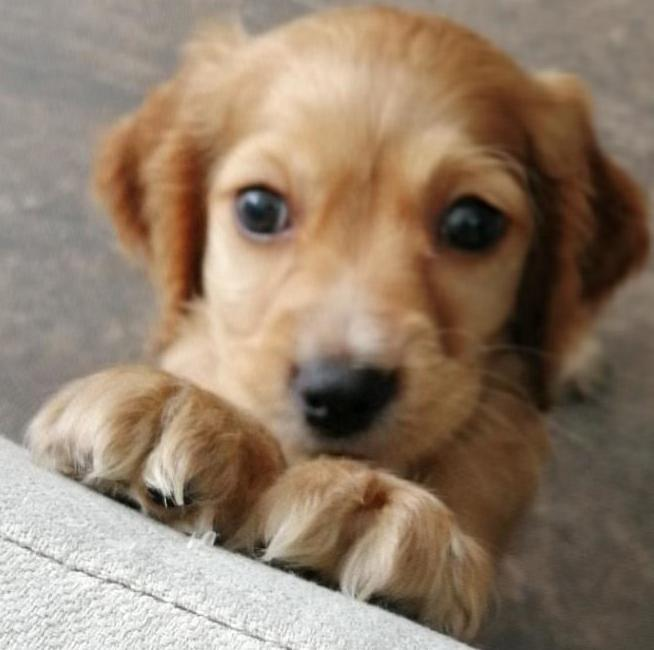
\includegraphics{blipf100.jpg}

The author cannot appreciate any difference between this picture and the
original one.

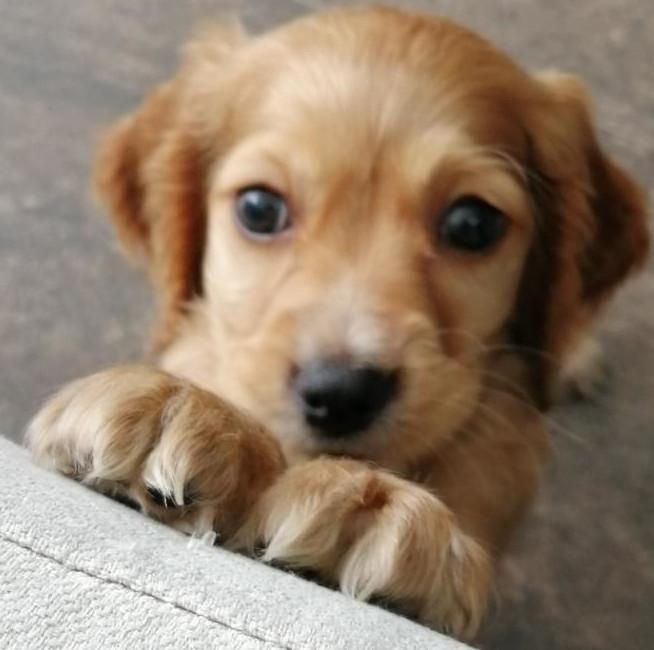
\includegraphics{blipf325.jpg}

As above the author cannot appreciate any difference between this
picture and the original one. note that this image uses almost the same
amount of information than the original one.

\hypertarget{final-thoughts}{%
\subsection{Final Thoughts}\label{final-thoughts}}

The image compression when used on a image has to have a rounding effect
due to the numbers used need to be integers. When checking the rounded
matrices for their rank the rounding process makes them behave like full
rank matrices, however checking the unrounded matrices gives the
expected results.

I seems that a 30\% compression is a sweet spot between an almost
identical image and small information size.

\end{document}
